% Chapter 6 — GPU Architecture, CUDA Programming, and Maximizing Occupancy  (v2: narrative edition)
% 53 pages; Part I follows the BOOK section order (SM internals -> threads/warps/blocks/grids -> limits -> PTX);
% 4 presenter intuition pages at 7, 9, 14, 15. Page numbers differ from v1. Use chapter06-lecture-script-v2-zh.md.
% v2 changes: book-plan opening (p2: SIMT -> CUDA -> memory -> roofline), question-driven roadmap (p3), worked-example p14, takeaway titles,
% unified workshop metaphor, occupancy caveat at p16, part-transition bridges, Plain-English takeaway bars.
% Compile: pdflatex chapter06-presentation-v2.tex  (run twice)
\documentclass[aspectratio=169]{beamer}

% ====== Presenter info: EDIT ME ======
\newcommand{\PresenterName}{Tianqin Cai}          % <-- 改成你的名字
\newcommand{\PresenterTitle}{Applied Scientist} % <-- 改成你的头衔
\newcommand{\PresenterOrg}{AWS}
% =====================================

\usetheme{Madrid}
\definecolor{navy}{RGB}{18,47,90}
\definecolor{kwblue}{RGB}{0,56,132}
\definecolor{okgreen}{RGB}{80,130,20}
\usecolortheme[named=navy]{structure}
\setbeamercolor{frametitle}{bg=navy,fg=white}
\setbeamercolor{title}{bg=navy,fg=white}
\setbeamercolor{block title}{bg=navy,fg=white}
\setbeamercolor{block body}{bg=gray!12,fg=black}
\setbeamercolor{block title example}{bg=okgreen,fg=white}
\setbeamercolor{block body example}{bg=okgreen!10,fg=black}
\setbeamertemplate{navigation symbols}{}
\setbeamertemplate{blocks}[rounded][shadow=true]

\usepackage{booktabs}
\usepackage{listings}
\lstset{
  language=C++,
  basicstyle=\ttfamily\fontsize{6.5}{7.6}\selectfont,
  keywordstyle=\color{kwblue}\bfseries,
  commentstyle=\color{gray}\itshape,
  stringstyle=\color{okgreen},
  showstringspaces=false,
  breaklines=true,
  columns=fullflexible
}

\newcommand{\kw}[1]{\textbf{\textcolor{kwblue}{#1}}}
\newcommand{\pe}[1]{\par{\setlength{\fboxsep}{2.5pt}\noindent\colorbox{navy!9}{\parbox{\dimexpr\textwidth-5pt\relax}{\footnotesize\itshape Plain English: #1}}}}
\newcommand{\bridge}[1]{{\footnotesize\itshape\textcolor{gray}{#1}}\par}
\newcommand{\refmark}[1]{\textsuperscript{[#1]}}

\title[AI Systems Performance Engineering]{AI Systems Performance Engineering}
\subtitle{Chapter 6 --- GPU Architecture, CUDA Programming, and Maximizing Occupancy}
\author[\PresenterName\ \ \PresenterTitle\ \ \PresenterOrg]{\PresenterName\\\PresenterTitle\\\PresenterOrg}
\institute[]{\footnotesize Internal Training for Applied Scientists on AI Infrastructure}
\date{August 15, 2026}

\begin{document}

% ================================================================ 1
\begin{frame}
  \titlepage
\end{frame}

% ================================================================ 2
\begin{frame}{What This Chapter Covers}
  \begin{enumerate}
    \item \kw{SIMT execution model} --- how \kw{warps}, \kw{thread blocks}, and \kw{grids}
          map your algorithm onto \kw{SMs}. \hfill (Part I)
    \item \kw{CUDA programming patterns} --- kernel anatomy, launch parameters,
          asynchronous allocation. \hfill (Part II)
    \item \kw{Memory hierarchy} --- register file, shared/L1, L2, HBM3e, plus
          asynchronous data movement (\kw{TMA}, \kw{TMEM}). \hfill (Part III)
    \item \kw{Roofline analysis} --- is a kernel \kw{compute-bound} or \kw{memory-bound}?
          Push toward \kw{peak throughput}. \hfill (Parts IV--V)
  \end{enumerate}
  \medskip
  \begin{block}{Where does occupancy fit?}
    \small Occupancy is the working metric that connects the SIMT model (Part I) to peak
    throughput (Parts IV--V): enough \kw{resident warps} keep SMs busy while data moves.
  \end{block}
  \pe{the arc: \kw{how the GPU executes} $\to$ how you program it $\to$ where data lives $\to$ \kw{what limits speed}.}
\end{frame}

% ================================================================ 3
\begin{frame}{Roadmap: Five Parts, Each Answers One Question}
  \begingroup\small\setlength{\tabcolsep}{6pt}\renewcommand{\arraystretch}{1.25}
  \begin{tabular}{@{}lll@{}}
    \toprule
    \textbf{Part} & \textbf{Slides} & \textbf{The question it answers} \\
    \midrule
    I \ GPU architecture & 4--20 & How does \kw{SIMT} map warps/blocks/grids onto SMs? \\
    II \ CUDA programming & 21--28 & How do we \kw{map a computation onto GPU threads}? \\
    III \ Memory hierarchy & 29--37 & Where does data \kw{live}, and what does \kw{movement cost}? \\
    IV \ Occupancy in practice & 38--46 & \kw{When} do more warps actually help? \\
    V \ Correctness \& roofline & 47--50 & Optimize \kw{compute} next, or \kw{memory}? \\
    \bottomrule
  \end{tabular}\endgroup
  \bigskip
  \begin{block}{The whole chapter in one sentence}
    \centering \kw{Expose enough parallelism, keep data close, and profile the real bottleneck.}
  \end{block}
  \medskip
  \centering\footnotesize\itshape
  When a detail page appears (SFU, TMEM, Unified Memory\ldots), it always belongs to one of these five questions.
\end{frame}

% ================================================================ 4
\begin{frame}{Part I --- GPUs Optimize Throughput; CPUs Optimize Latency}
  \begin{columns}[c]
    \column{0.55\textwidth}
    \begin{itemize}
      \item CPUs: few cores, deep caches, fast \emph{single} threads. GPUs: hundreds of \kw{SMs}
            (streaming multiprocessors) running \kw{thousands of threads} in parallel.
      \item Basic CUDA flow (right): host copies data \kw{CPU $\to$ GPU}, launches a \kw{kernel},
            copies results back.
      \item The GPU's edge is \kw{massive parallelism}: many SMs process different data
            \kw{at once}; within an SM, \kw{resident warps} also fill memory stalls.
      \item Sweet spot: \kw{data-parallel} work --- matrix multiplies, convolutions ---
            written in CUDA C++ or via \kw{PyTorch} / OpenAI \kw{Triton}.\refmark{1,3}
    \end{itemize}
    \column{0.42\textwidth}
    \centering
    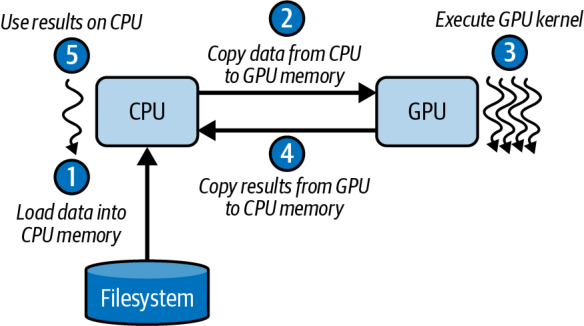
\includegraphics[width=0.88\linewidth]{figs/fig6-1.png}\\
    {\scriptsize Figure 6-1. Simple CUDA programming flow}
  \end{columns}
  \pe{the CPU finishes one part fast; the GPU is a \kw{factory} --- keep \kw{every workshop busy}.}
\end{frame}

% ================================================================ 5
\begin{frame}{Inside a Blackwell SM: The Resource Budget}
  \begin{columns}[c]
    \column{0.52\textwidth}
    \begin{itemize}
      \item Each SM tracks up to \kw{64 warps} (\kw{warp} = 32 threads; details p.~13)
            = \kw{2{,}048 threads} --- the pool the scheduler switches between.
      \item \kw{64K 32-bit registers} per SM (256 KB total); any single thread can use
            at most \kw{255}.
      \item \kw{256 KB} combined L1 cache / shared memory; up to \kw{228 KB} configurable as
            user-managed shared memory (\kw{227 KB usable} --- CUDA reserves 1 KB per block).
      \item These on-chip budgets let one SM juggle thousands of threads without
            constantly touching DRAM.\refmark{2}
    \end{itemize}
    \column{0.45\textwidth}
    \centering
    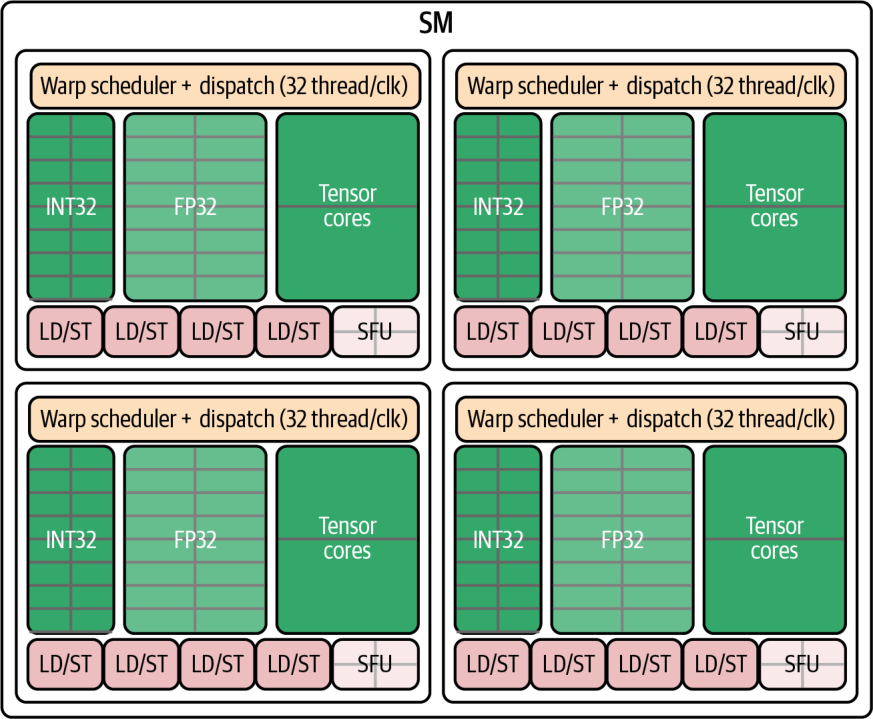
\includegraphics[width=0.8\linewidth]{figs/fig6-2.png}\\
    {\scriptsize Figure 6-2. A Blackwell SM: four scheduling partitions sharing on-chip resources}
  \end{columns}
  \pe{an SM is a workshop: registers are toolbelts, shared memory is the workbench.}
\end{frame}

% ================================================================ 6
\begin{frame}{SFUs and Load/Store Pipelines}
  \begin{columns}[t]
    \column{0.48\textwidth}
    \begin{block}{SFU --- Special Function Unit}
      \begin{itemize}\small
        \item Handles \kw{transcendentals}: sine, cosine, reciprocal, square root.
        \item Own \kw{dedicated pipeline} --- \emph{not} part of the dual-issue math+memory pair (p.~8).
        \item Slow functions never stall the core compute/memory pipes $\Rightarrow$
              more \kw{instruction-level parallelism} for mixed-operation kernels.
      \end{itemize}
    \end{block}
    \column{0.48\textwidth}
    \begin{block}{LD/ST --- Load/Store pipelines}
      \begin{itemize}\small
        \item \kw{16 LD/ST pipelines} per SM (4 per scheduler) feed L1/shared, L2, and global memory.
        \item \kw{Caveat (book warning):} exact counts and pairings are \kw{not guaranteed} ---
              rely on profiling counters and the \kw{Blackwell tuning guide}.\refmark{2}
      \end{itemize}
    \end{block}
  \end{columns}
  \pe{the SFU is a specialist counter at the back of the store --- complicated requests go there so the express lanes keep moving.}
\end{frame}

% ================================================================ 7
\begin{frame}{Two Views of One Machine: Software vs.\ Hardware}
  \begin{columns}[c]
    \column{0.56\textwidth}
    {\footnotesize\setlength{\tabcolsep}{2pt}
    \begin{tabular}{@{}lll@{}}
      \toprule
      \textbf{Software (you write)} & \textbf{Hardware (runs it)} & \textbf{Analogy} \\
      \midrule
      Grid & \kw{all SMs} & the batch of orders \\
      Block & \kw{one SM} (for life) & one work team \\
      \emph{(warp: implicit)} & the issue unit & 32-worker crew \\
      Thread & one lane of a warp & one worker \\
      \bottomrule
    \end{tabular}}\\[6pt]
    \begin{itemize}\small
      \item You choose \kw{grid and block sizes}; hardware decides placement and
            scheduling. A block \kw{never migrates} --- but one SM usually
            \kw{hosts several blocks}.
      \item The \kw{warp is the bridge}: hardware slices every block into
            warps of 32 --- automatically, invisibly.
      \item Memory preview (Part III): registers = toolbox, shared = workbench,
            L1 = shop shelf, \kw{L2 = central depot}, \kw{HBM = warehouse};
            a global load tries L1 $\to$ L2 $\to$ HBM and returns the same way.
    \end{itemize}
    \column{0.40\textwidth}
    \centering
    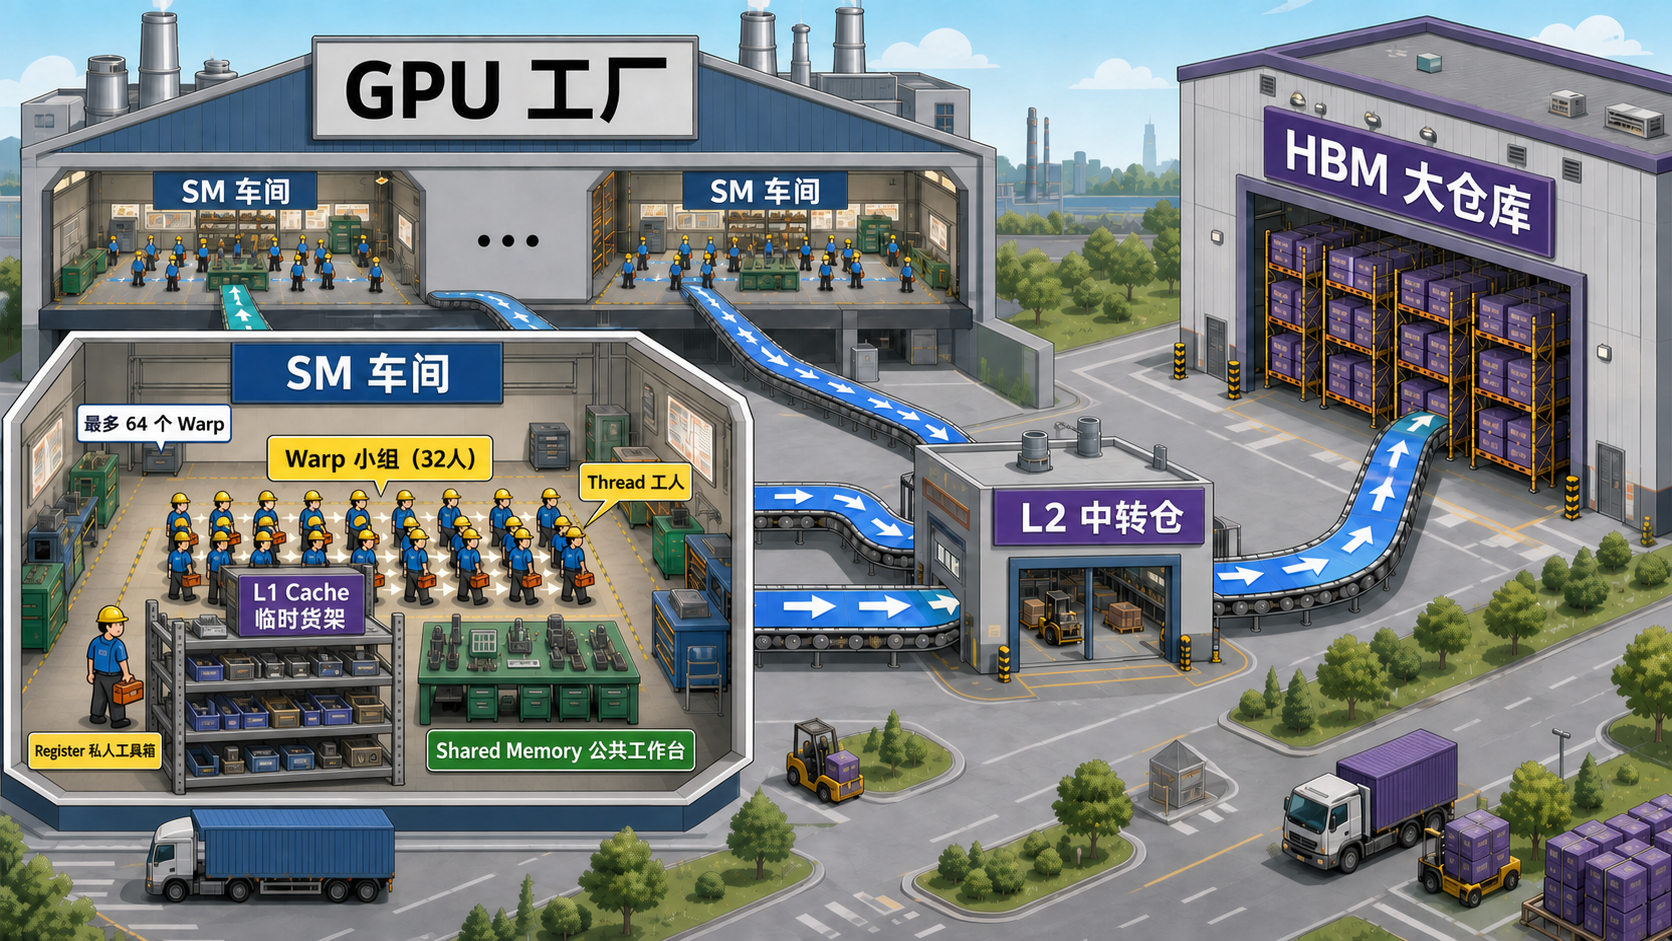
\includegraphics[width=\linewidth]{figs/analogy-gpu-factory.png}\\
    {\scriptsize Presenter's analogy: SM workshops, L2 depot, HBM warehouse}
  \end{columns}
  \pe{software speaks in \kw{grids and blocks}; hardware answers in \kw{SMs and warps} --- the warp is where they meet.}
\end{frame}

% ================================================================ 8
\begin{frame}{Four Warp Schedulers, Dual Issue}
  \begin{columns}[c]
    \column{0.58\textwidth}
    \begin{itemize}
      \item Each SM = four ``\kw{mini-SMs}'': independent warp schedulers with their own dispatch logic.
      \item Each scheduler issues \kw{1 warp instruction per cycle} $\Rightarrow$ up to
            \kw{4 warps advance per cycle}.
      \item \kw{Dual-issue}: one math (INT32/FP32/Tensor Core) \kw{+} one memory (load/store)
            instruction per cycle --- \emph{from the same warp}, never across warps.
      \item Best case: \kw{4 math + 4 memory} instructions in flight every cycle.
    \end{itemize}
    \column{0.38\textwidth}
    \centering
    {\small
    \begin{tabular}{@{}ll@{}}
      \toprule
      \textbf{Per cycle (Table 6-1)} & \textbf{Limit} \\
      \midrule
      Schedulers & 4 \\
      Warps issued & 4 \\
      Math / memory ops & 4 / 4 \\
      \bottomrule
    \end{tabular}}\\[6pt]
    {\scriptsize Book note: table values are illustrative;\\real benchmarks in the GitHub repo\refmark{7}}
  \end{columns}
  \pe{\kw{four dispatchers} on one floor, each sending out one crew per beat --- and a crew can compute with one hand while fetching parts with the other.}
\end{frame}

% ================================================================ 9
\begin{frame}{Analogy: One SM Is a Workshop}
  \begin{columns}[c]
    \column{0.54\textwidth}
    \centering
    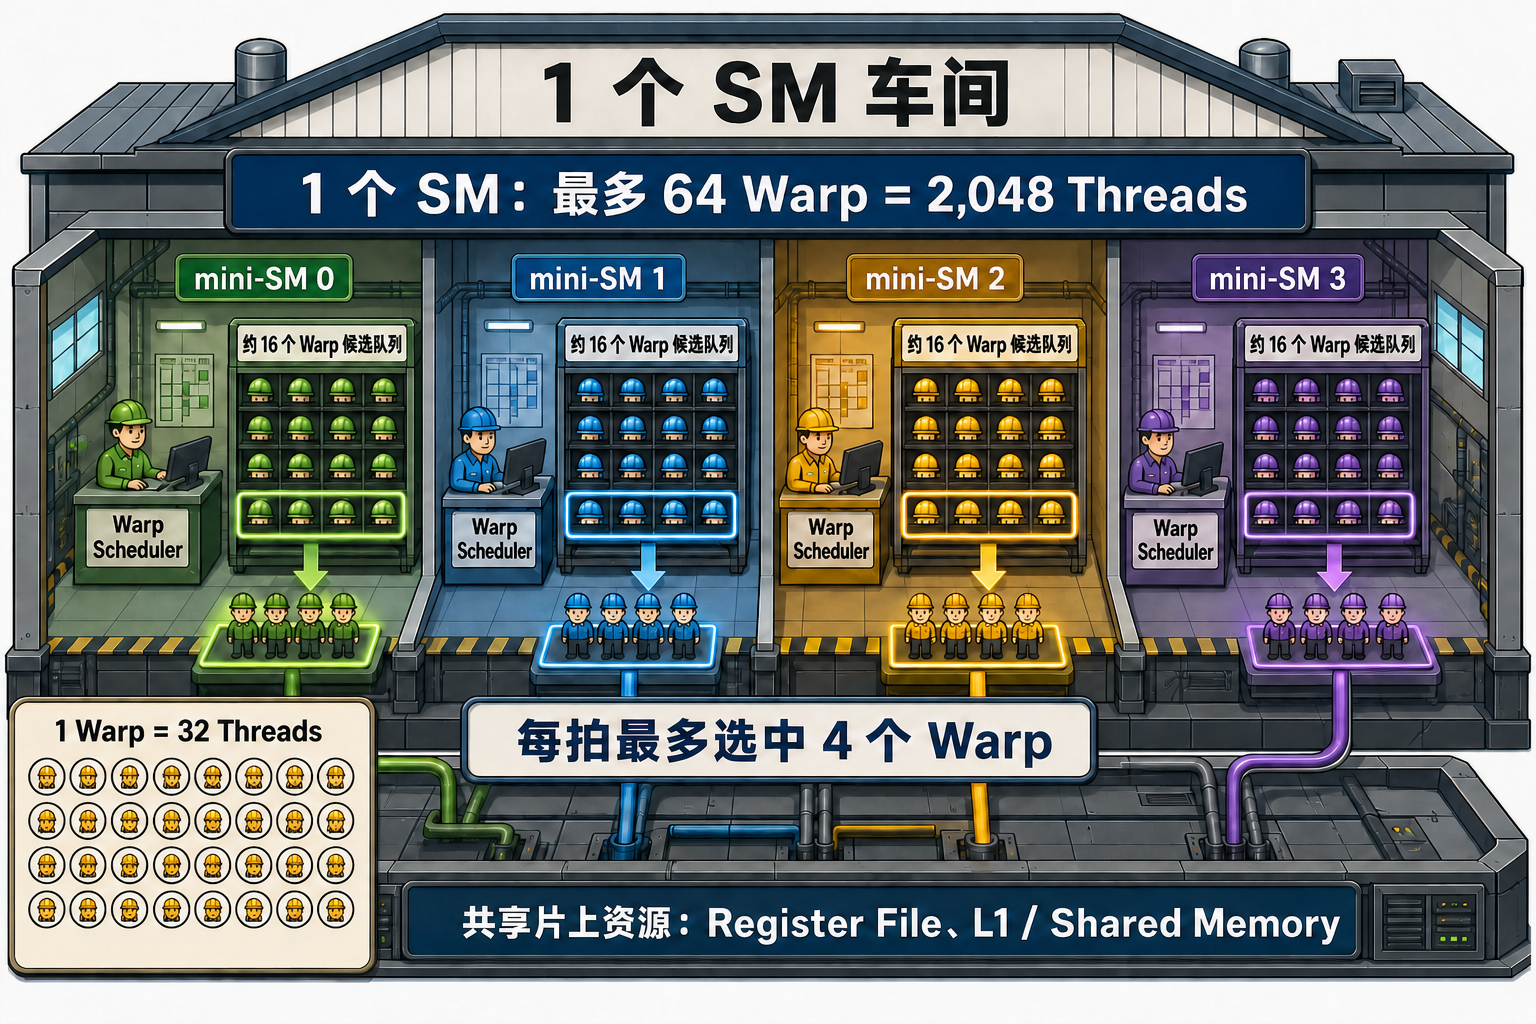
\includegraphics[width=0.86\linewidth]{figs/analogy-sm-workshop.png}\\
    {\scriptsize Presenter's analogy figure (not from the book)}
    \column{0.44\textwidth}
    \begin{itemize}\footnotesize
      \item Four bays = \kw{4 scheduling partitions} (``mini-SMs''), one
            \kw{warp scheduler} each --- CUDA only ever sees the whole SM.
      \item Hard hats on shelves = \kw{resident warps}: $\sim$16 per partition, \kw{64 total}.
            Resident = state already allocated --- \emph{not} ``executing right now.''
      \item Highlighted crews = the \kw{$\leq$4 warps issued this cycle}
            (each scheduler picks at most 1 \emph{ready} warp).
      \item Bottom left: \kw{1 warp = 32 threads} --- dispatched as a whole crew.
      \item Common foundation: \kw{register file, L1, shared memory} ---
            shared by all four partitions.
    \end{itemize}
  \end{columns}
  \pe{64 crews on standby, 4 dispatchers, at most 4 crews per beat --- each crew is 32 workers.}
\end{frame}

% ================================================================ 10
\begin{frame}{The Thread Hierarchy: Threads $\to$ Blocks $\to$ Grids}
  \begin{columns}[c]
    \column{0.52\textwidth}
    \begin{itemize}
      \item \kw{Thread}: runs your kernel code on one data element.
      \item \kw{Thread block} (CTA --- cooperative thread array): up to \kw{1{,}024 threads};
            shares fast on-chip \kw{shared memory}.
      \item \kw{Grid}: all blocks of one launch --- sized right, it scales to
            \kw{millions of threads} with zero kernel changes.
      \item The CUDA runtime (and PyTorch) handles scheduling and distribution across all SMs.
    \end{itemize}
    \column{0.45\textwidth}
    \centering
    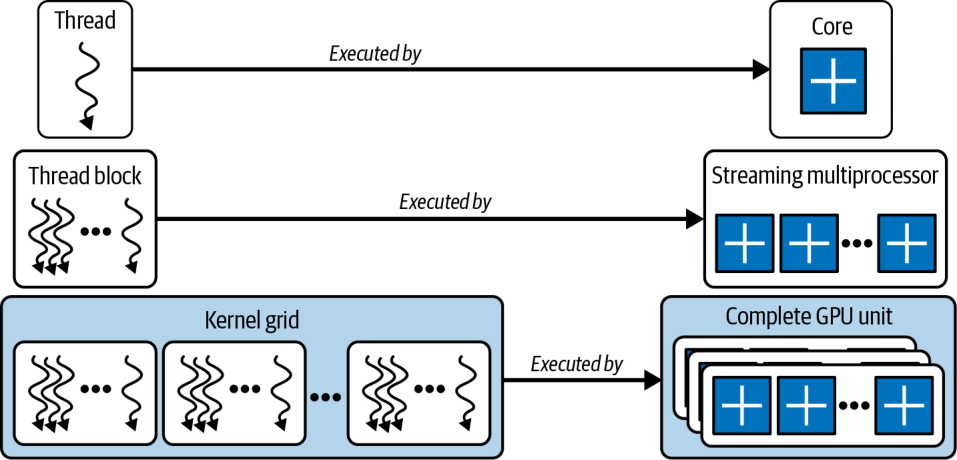
\includegraphics[width=\linewidth]{figs/fig6-3.png}\\
    {\scriptsize Figure 6-3. Threads, thread blocks (CTAs), and grids}
  \end{columns}
  \pe{workers (threads) form teams (blocks) that talk cheaply inside the team; the company (grid) hires as many teams as the job needs.}
\end{frame}

% ================================================================ 11
\begin{frame}{Blocks Cooperate Inside, Stay Independent Outside}
  \begin{columns}[c]
    \column{0.52\textwidth}
    \begin{itemize}
      \item Within a block: share data via shared memory, synchronize with
            \kw{\texttt{\_\_syncthreads()}} (a barrier: everyone arrives before anyone continues).
      \item \kw{Every barrier costs time} --- the book's advice: \kw{minimize synchronization points}.
      \item Across blocks: \kw{independent, no guaranteed order}. That freedom lets the scheduler
            spray blocks over all SMs --- and lets your kernel run \kw{unmodified on future GPUs}
            with more SMs.
    \end{itemize}
    \column{0.45\textwidth}
    \centering
    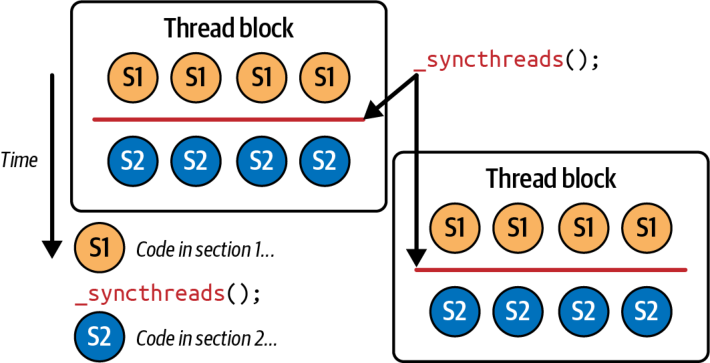
\includegraphics[width=0.9\linewidth]{figs/fig6-6.png}\\
    {\scriptsize Figure 6-6. \texttt{\_\_syncthreads()} between two code sections}
  \end{columns}
  \pe{team huddles (barriers) are useful but expensive --- call as few as possible; and never assume team A finishes before team B.}
\end{frame}

% ================================================================ 12
\begin{frame}{Thread Block Clusters and DSMEM}
  \begin{columns}[c]
    \column{0.52\textwidth}
    \begin{itemize}\small
      \item Traditionally, threads in \emph{different} blocks could not cooperate. Modern GPUs add
            \kw{thread block clusters}: blocks that communicate \kw{across SMs},
            with cluster-scoped hardware barriers.
      \item Backed by \kw{DSMEM} (distributed shared memory): the shared-memory banks of
            participating SMs, linked over a fast \kw{on-chip interconnect} into one pool.
      \item Threads read, write, and atomically update each other's shared buffers
            \kw{at on-chip speeds --- without global-memory bandwidth}.
      \item Key enabler for huge matmuls in LLMs --- details in \kw{Chapter 10}.
    \end{itemize}
    \column{0.45\textwidth}
    \centering
    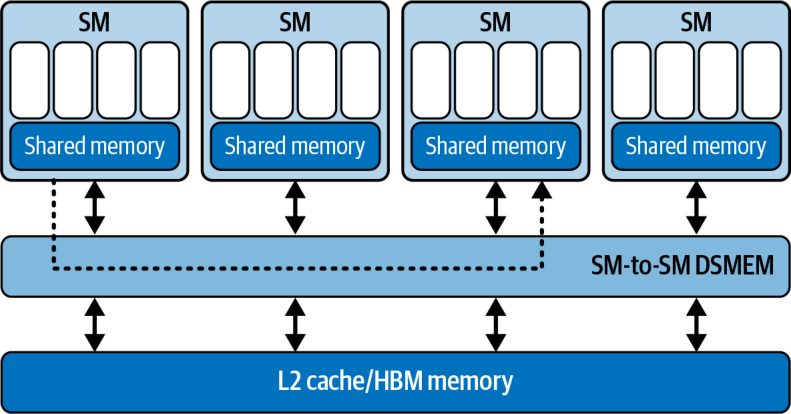
\includegraphics[width=\linewidth]{figs/fig6-5.png}\\
    {\scriptsize Figure 6-5. DSMEM shared across thread blocks in a cluster}
  \end{columns}
  \pe{neighboring teams knock a door through the wall between their workbenches instead of mailing parts through the warehouse.}
\end{frame}

% ================================================================ 13
\begin{frame}{Warps and SIMT: 32 Threads in Lockstep}
  \begin{columns}[c]
    \column{0.52\textwidth}
    \begin{itemize}
      \item Blocks are subdivided into \kw{warps of 32 threads} that execute one instruction
            together under \kw{SIMT} (single instruction, multiple threads).
      \item The warp --- not the thread --- is what the \kw{hardware actually schedules};
            warp size has been \kw{32 on every GPU generation}.
      \item The hardware hides long-latency events (global loads, cache fills, pipeline stalls)
            by \kw{rapidly switching among warps}.
    \end{itemize}
    \column{0.45\textwidth}
    \centering
    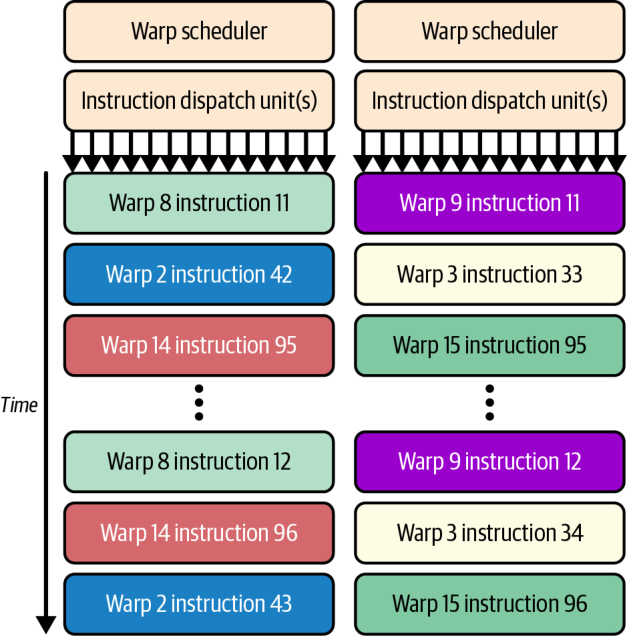
\includegraphics[width=0.8\linewidth]{figs/fig6-7.png}\\
    {\scriptsize Figure 6-7. A warp advances as a whole under the warp scheduler}
  \end{columns}
  \pe{a warp is a \kw{32-worker crew}: one instruction for all 32, everyone moves together --- or the whole crew waits.}
\end{frame}

% ================================================================ 14
\begin{frame}{Worked Example: One Million Adds Through Both Views}
  \begin{columns}[t]
    \column{0.46\textwidth}
    \begin{block}{Software view: you write the order sheet}
      \footnotesize
      \texttt{add<<<3907, 256>>>(A, B, C, N);}\\[4pt]
      {\scriptsize\setlength{\tabcolsep}{3pt}
      \begin{tabular}{@{}ll@{}}
        \toprule
        Grid & 1 (this launch) \\
        Blocks & \kw{3{,}907} $= \lceil 10^6/256 \rceil$ \\
        Threads / block & \kw{256} (your choice) \\
        Warps / block & \kw{8} (= 256 $\div$ 32, HW slices) \\
        Total & $\sim$1M threads, 31{,}256 warps \\
        \bottomrule
      \end{tabular}}\\[4pt]
      Each thread only says: ``I handle element \texttt{idx}.''
    \end{block}
    \column{0.50\textwidth}
    \begin{block}{Hardware view: toy GPU --- 4 SMs, 2 blocks/SM}
      \footnotesize
      \begin{enumerate}
        \item First \kw{8 blocks} move in: 2 per SM.
        \item Each SM now holds $2 \times 8 = $ \kw{16 resident warps}.
        \item Schedulers keep issuing whichever warps are \kw{ready} (= latency hiding --- next page).
        \item A block finishes $\Rightarrow$ the next of the \kw{3{,}899 waiting} blocks
              moves in --- batch by batch until all 3{,}907 are done.
      \end{enumerate}
    \end{block}
  \end{columns}
  \smallskip
  \begin{itemize}\footnotesize
    \item 4 SMs or 400 SMs: \kw{same code} --- the grid \kw{decouples} the program from the GPU's size.
  \end{itemize}
  \pe{you write the \kw{order sheet} (3,907 teams of 256 workers); the hardware assigns teams to workshops and slices each team into 32-worker crews.}
\end{frame}

% ================================================================ 15
\begin{frame}{Let the Workshop Move: Latency Hiding, Cycle by Cycle}
  \begin{columns}[t]
    \column{0.48\textwidth}
    \begin{block}{One partition, one moment}
      \small
      Warp A --- \kw{waiting} on an HBM load\\
      Warp B --- \kw{waiting} on a previous result\\
      Warp C --- \kw{ready}\qquad Warp D --- \kw{ready}\\[4pt]
      The scheduler skips A and B and \kw{issues C or D} ---
      skipping a stalled warp costs \kw{nothing}.
    \end{block}
    {\small
    \begin{tabular}{@{}ll@{}}
      \toprule
      \textbf{Cycle} & \textbf{Issued (example)} \\
      \midrule
      1 & Warp C \\
      2 & Warp F \\
      3 & Warp D \\
      4 & Warp H \\
      \bottomrule
    \end{tabular}}
    \column{0.48\textwidth}
    \begin{itemize}
      \item ``Issued'' = the instruction \kw{starts}; it need not finish this cycle.
      \item Latency hiding does \kw{not} shorten any warp's wait ---
            it \kw{fills the wait} with other warps' work.
      \item This is why \kw{64 resident warps} matter: a deep pool of \emph{ready}
            candidates for the 4 dispatchers --- and why low occupancy hurts
            (nothing ready to switch to).
    \end{itemize}
  \end{columns}
  \pe{latency hiding does \kw{not} reduce waiting time --- it \kw{fills the waiting time} with other crews' work.}
\end{frame}

% ================================================================ 16
\begin{frame}{Occupancy Gives the Scheduler More Choices}
  \begin{block}{Definition}
    \kw{Occupancy} = active warps on an SM $\div$ the hardware maximum (64 on Blackwell).
    ``\kw{Achieved occupancy}'' is the measured average, reported by Nsight Compute.
  \end{block}
  \begin{columns}[t]
    \column{0.48\textwidth}
    \begin{itemize}
      \item High occupancy $\Rightarrow$ when one warp stalls on memory, another is ready
            $\Rightarrow$ \kw{latency hiding}.
      \item Blackwell's large register file (64K/SM) makes high occupancy easier to reach.
    \end{itemize}
    \column{0.48\textwidth}
    \begin{itemize}
      \item The counterweight: warps share \kw{registers and shared memory}. Pack in too many
            $\Rightarrow$ \kw{register spilling} to slow memory --- a new stall you created.
      \item So: profile occupancy \kw{together with} register / shared-memory usage.
    \end{itemize}
  \end{columns}
  \pe{occupancy is \kw{not} ``how busy the GPU is'' and \kw{not} a performance score --- it counts \kw{how many resident crews the dispatcher can choose from}. Enough hides latency; beyond enough, more may not help (p.~52).}
\end{frame}

% ================================================================ 17
\begin{frame}{Warp Divergence: When {\ttfamily if/else} Splits the Crew}
  \begin{columns}[c]
    \column{0.52\textwidth}
    \begin{itemize}
      \item If threads \emph{within one warp} take different branches, the warp \kw{serializes}:
            it runs the \texttt{if} path with the other lanes \kw{masked}, then the \texttt{else} path.
      \item Execution time multiplies by the \kw{number of distinct paths}.
      \item \kw{No penalty across warps} --- different warps may branch differently for free.
      \item Practical corollary: branch on \kw{warp-aligned} conditions
            (\texttt{threadIdx.x / 32}), not per-thread parity (\texttt{threadIdx.x \% 2}).
      \item Detection and mitigation: Chapter 8 (Nsight Compute).
    \end{itemize}
    \column{0.45\textwidth}
    \centering
    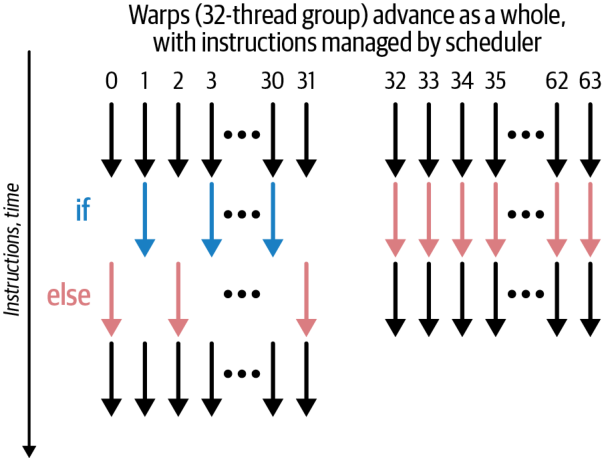
\includegraphics[width=0.76\linewidth]{figs/fig6-8.png}\\
    {\scriptsize Figure 6-8. SIMT warp divergence (left) vs.\ uniformity (right)}
  \end{columns}
  \pe{if half the \kw{crew} takes one work order and half another, the crew runs \kw{each job twice}.}
\end{frame}

% ================================================================ 18
\begin{frame}{Hardware Limits I: Warp and Block (Table 6-2)}
  \bridge{No need to memorize these numbers. The one idea: each block's threads, registers, and shared memory decide how many blocks and warps still fit on one SM.}
  \begin{columns}[c]
    \column{0.52\textwidth}
    {\small
    \begin{tabular}{@{}ll@{}}
      \toprule
      \textbf{Resource} & \textbf{Limit (B200)} \\
      \midrule
      Warp size & 32 threads \\
      Max threads / block & 1{,}024 \\
      Max warps / block & 32 \ (= 1024 $\div$ 32) \\
      \bottomrule
    \end{tabular}}\\[6pt]
    {\scriptsize \texttt{blockDim.x $\times$ blockDim.y $\times$ blockDim.z $\leq$ 1024}}
    \column{0.45\textwidth}
    \begin{block}{Why multiples of 32 matter}
      \small A \kw{33-thread block} occupies \kw{two} warp slots --- the second warp runs
      \kw{1 of 32 lanes} but still consumes a full scheduler slot. Every non-multiple of 32
      donates scheduler capacity to the void.
    \end{block}
  \end{columns}
  \medskip
  \begin{itemize}
    \item Block too big $\Rightarrow$ too many registers per block $\Rightarrow$ \kw{spilling};
          or too much shared memory (227 KB usable is shared by \kw{all resident blocks} on the SM).
    \item Smaller blocks can mean \kw{higher occupancy} --- more independent blocks fit per SM.
  \end{itemize}
\end{frame}

% ================================================================ 19
\begin{frame}{Hardware Limits II: SM-Resident and Grid (Tables 6-3 / 6-4)}
  \begin{columns}[c]
    \column{0.55\textwidth}
    {\small\setlength{\tabcolsep}{4pt}
    \begin{tabular}{@{}ll@{}}
      \toprule
      \textbf{Per SM (resident)} & \textbf{Limit} \\
      \midrule
      Max warps & \kw{64} (= 2{,}048 threads) \\
      Max threads & 2{,}048 \\
      Max blocks & 32 \\
      \midrule
      \textbf{Grid} & \\
      \midrule
      Max blocks (X / Y / Z) & $\sim$2.1B / 65{,}535 / 65{,}535 \\
      Max concurrent grids & \kw{128} kernels per device \\
      \bottomrule
    \end{tabular}}
    \column{0.42\textwidth}
    \centering
    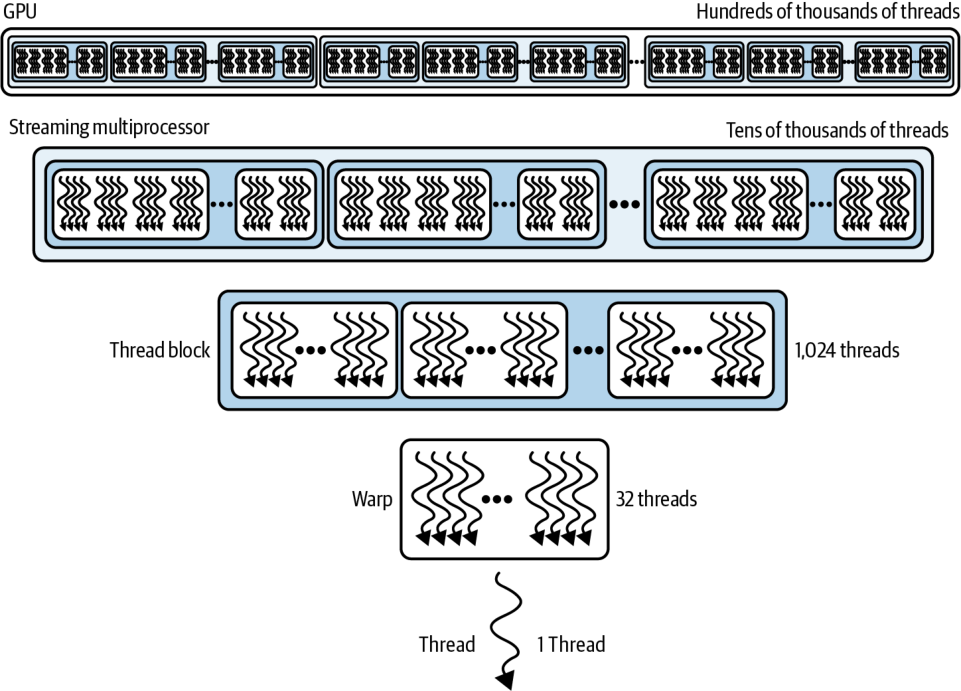
\includegraphics[width=\linewidth]{figs/fig6-9.png}\\
    {\scriptsize Figure 6-9. Relative scale of thread resources}
  \end{columns}
  \medskip
  \begin{itemize}\small
    \item Worked example: 1024-thread blocks $\Rightarrow$ only \kw{2 blocks/SM};
          256-thread blocks $\Rightarrow$ \kw{8 blocks/SM} --- same 2{,}048 threads, more flexibility.
    \item In practice you hit \kw{per-SM limits} long before grid limits;
          $>$65{,}535 blocks in Y/Z $\Rightarrow$ use 2D/3D grids or multilaunch.\refmark{1,2}
  \end{itemize}
\end{frame}

% ================================================================ 20
\begin{frame}{Compatibility: PTX, SASS, and Fatbins}
  \begin{columns}[t]
    \column{0.48\textwidth}
    \begin{itemize}
      \item \kw{SASS}: final machine code for \emph{one} architecture (sm\_90 = Hopper,
            sm\_100 = Blackwell). SASS-only binaries \kw{won't run on newer GPUs}.
      \item \kw{PTX}: virtual ISA the driver \kw{JIT-compiles} at load time $\Rightarrow$
            \kw{forward compatibility}.
      \item Family targets (\texttt{sm\_100f}) restrict portability to the same feature family.
    \end{itemize}
    \column{0.48\textwidth}
    \begin{block}{Best practice}
      \small Ship a \kw{fatbin}: generic PTX \kw{+} the family-specific cubins you need for
      optimizations --- with \kw{fallback paths} for other architectures.
    \end{block}
    \begin{itemize}\small
      \item Verify with \kw{\texttt{CUDA\_FORCE\_PTX\_JIT=1}}: forces PTX JIT;
            if the binary lacks PTX, \kw{kernel launch fails} --- rebuild with PTX.
    \end{itemize}
  \end{columns}
  \pe{fast code must also \kw{survive GPU generations} --- ship optimized \kw{SASS} for today's chips plus \kw{PTX} for forward compatibility.}
\end{frame}

% ================================================================ 21
\begin{frame}[fragile]{Part II --- Anatomy of a CUDA Kernel: Device Side}
  \bridge{The hardware wants many ready warps --- now: how does CUDA code create them?}
  \begin{columns}[t]
    \column{0.52\textwidth}
\begin{lstlisting}[emph={blockIdx,blockDim,threadIdx,idx},emphstyle=\color{kwblue}\bfseries]
__global__ void myKernel(float* input, int N) {
    // unique global index for this thread
    int idx = blockIdx.x * blockDim.x + threadIdx.x;
    if (idx < N) {          // bounds check!
        input[idx] *= 2.0f; // in-place: double it
    }
}
\end{lstlisting}
    \begin{itemize}\small
      \item \kw{\texttt{\_\_global\_\_}}: runs on the device, callable from the host.
      \item Built-ins: \texttt{blockIdx} (which block am I), \texttt{blockDim} (block size),
            \texttt{threadIdx} (my rank in the block).
    \end{itemize}
    \column{0.44\textwidth}
    \begin{itemize}
      \item The kernel is written from the perspective of \kw{one thread};
            \texttt{idx} carves out its slice of the data.
      \item CUDA compiles it into device code executed by \kw{thousands or millions}
            of lightweight threads in parallel.
      \item Launch syntax (host): \kw{\texttt{<<<blocksPerGrid, threadsPerBlock>>>}} ---
            the two core parameters of \emph{every} kernel invocation.
    \end{itemize}
  \end{columns}
  \pe{write the job description for \emph{one} worker; CUDA prints a million copies, each with a different row number.}
\end{frame}

% ================================================================ 22
\begin{frame}[fragile]{Host Side: The Six-Step Data Flow}
  \begin{columns}[t]
    \column{0.55\textwidth}
\begin{lstlisting}
const int N = 1'000'000;
float *h_input = nullptr, *d_input = nullptr;   // h_=host, d_=device
cudaMallocHost(&h_input, N * sizeof(float));    // 1) pinned host alloc
for (int i = 0; i < N; ++i) h_input[i] = 1.0f;  //    init
cudaMalloc(&d_input, N * sizeof(float));        //    device alloc
cudaMemcpy(d_input, h_input, N * sizeof(float),
           cudaMemcpyHostToDevice);             // 2) H2D copy
const int threadsPerBlock = 256;
const int blocksPerGrid =                       //    = 3,907 for 1M
    (N + threadsPerBlock - 1) / threadsPerBlock;
myKernel<<<blocksPerGrid, threadsPerBlock>>>(d_input, N); // 3) launch
cudaDeviceSynchronize();                        // 4) wait for device
cudaMemcpy(h_input, d_input, N * sizeof(float),
           cudaMemcpyDeviceToHost);             // 5) D2H copy
cudaFree(d_input); cudaFreeHost(h_input);       // 6) cleanup
\end{lstlisting}
    \column{0.42\textwidth}
    \begin{itemize}
      \item Naming convention: \kw{\texttt{h\_}} = host pointer, \kw{\texttt{d\_}} = device pointer
            --- used throughout the book.
      \item \kw{\texttt{cudaMallocHost}} = \kw{pinned} (page-locked) memory ---
            prerequisite for async copies to truly overlap later.
      \item Book note: \emph{not fully optimized yet} --- this is the simple, complete
            \kw{template} the rest of the book improves on.
    \end{itemize}
  \end{columns}
\end{frame}

% ================================================================ 23
\begin{frame}{Why Pass N? The Single-Thread Perspective}
  \begin{block}{The book's answer}
    ``A CUDA kernel function is designed to work \kw{inside of a single thread}, alongside thousands
    of other threads, \kw{on a partition of the input data}. As such, N defines the size of the
    partition that this particular kernel will process.''
  \end{block}
  \begin{itemize}
    \item A CPU function could just inspect the array size. A kernel \kw{cannot} ---
          it sees a raw pointer and must be told where its world ends.
    \item Combined with \texttt{blockIdx}/\texttt{blockDim}/\texttt{threadIdx}, N lets every
          element be processed \kw{cleanly and uniquely}, in parallel, across many SMs.
    \item This is the core mental shift from CPU to GPU programming: you don't write
          ``process the array,'' you write ``process \kw{my} element --- if it exists.''
  \end{itemize}
  \pe{each of the million copied workers gets the same memo; N is the line that says where the job ends.}
\end{frame}

% ================================================================ 24
\begin{frame}{The Bounds Check --- and Lazily Surfacing Errors}
  \begin{columns}[t]
    \column{0.5\textwidth}
    \begin{block}{Worked example: N = 63}
      \small Scheduler assigns \kw{2 warps} (64 threads). Warp 1 handles elements 0--31 --- fine.
      Warp 2 expects 32--63 \kw{plus one extra thread}; without \texttt{if (idx < N)} it reads
      past the array $\Rightarrow$ \kw{\texttt{cudaErrorIllegalAddress}}.
    \end{block}
    \begin{itemize}\small
      \item Book rule: bounds checks are everywhere in CUDA; ``if you don't see it,
            \kw{understand why it's not there}.''
    \end{itemize}
    \column{0.47\textwidth}
    \begin{itemize}
      \item Kernels run \kw{asynchronously, with no per-thread exceptions}: an illegal access sets a
            \kw{global fault flag} for the whole launch.
      \item The host only sees it at the \kw{next sync or CUDA API call} --- errors surface
            \kw{lazily}.
      \item Practice: \kw{\texttt{cudaGetLastError()} + \texttt{cudaDeviceSynchronize()}}
            right after launches, so faults are caught where they happen.
    \end{itemize}
  \end{columns}
  \pe{the GPU doesn't call you when something breaks --- it leaves a note you only find the next time you check the mailbox.}
\end{frame}

% ================================================================ 25
\begin{frame}{Choosing Launch Parameters: The 256 Recipe}
  \begin{block}{Recipe that works almost everywhere}
    Start with \kw{\texttt{threadsPerBlock = 256}} (8 warps);
    \kw{\texttt{blocksPerGrid = (N + 255) / 256}} (round up --- every element covered). Tune 128/512 by profiling.
  \end{block}
  \begin{itemize}
    \item \kw{Multiple of 32}: no half-empty warps occupying scheduler slots.
    \item \kw{Latency hiding}: hundreds of threads per SM cover DRAM and instruction stalls ---
          8 blocks $\times$ 256 = 2{,}048 \emph{can} fill an SM, \kw{if registers and shared memory allow}.
    \item \kw{Occupancy}: 8 warps/block usually fits registers and shared memory comfortably.
    \item \kw{Resource-balanced}: far from the 1{,}024 cap, big enough to keep warps busy.
    \item Book tip for Blackwell: consider \kw{256--512} threads per block.
  \end{itemize}
  \pe{256 is the ``medium coffee'' of block sizes --- almost never the wrong first order, refine later if profiling says so.}
\end{frame}

% ================================================================ 26
\begin{frame}[fragile]{2D and 3D Kernel Inputs}
  \begin{columns}[t]
    \column{0.52\textwidth}
\begin{lstlisting}
__global__ void my2DKernel(float* input,
                           int width, int height) {
    int x = blockIdx.x * blockDim.x + threadIdx.x;
    int y = blockIdx.y * blockDim.y + threadIdx.y;
    if (x < width && y < height) {  // 2D bounds check
        int idx = y * width + x;    // flatten to 1D
        input[idx] *= 2.0f;
    }
}
// host: dim3 threads(16,16);  // 256 threads, 2D
//       dim3 blocks((W+15)/16, (H+15)/16);
\end{lstlisting}
    \column{0.44\textwidth}
    \begin{itemize}
      \item Natural fit for \kw{images}: e.g., a $1{,}024 \times 1{,}024$ matrix processed by
            $16 \times 16$ blocks (still 256 threads).
      \item Same pattern generalizes to 3D with \kw{\texttt{dim3(x, y, z)}} ---
            volumetric data maps directly onto the thread hierarchy.
      \item Book note: most of the book uses \kw{1D or 2D (tiled)} launches;
            in 1D, plain ints beat \texttt{dim3}.
    \end{itemize}
  \end{columns}
  \pe{same recipe, two axes: each worker gets a (row, column) badge instead of a single row number.}
\end{frame}

% ================================================================ 27
\begin{frame}[fragile]{Allocate Asynchronously: Streams and Memory Pools}
  \begin{columns}[t]
    \column{0.52\textwidth}
\begin{lstlisting}
cudaStream_t s;
cudaStreamCreateWithFlags(&s, cudaStreamNonBlocking);

float* d_buf = nullptr;
cudaMallocAsync(&d_buf, N * sizeof(float), s);
myKernel<<<blocks, threads, 0, s>>>(d_buf, N);
cudaFreeAsync(d_buf, s);  // deferred until s finishes
\end{lstlisting}
    \begin{itemize}\small
      \item \kw{Free waits only for stream \texttt{s}} --- no global
            \texttt{cudaDeviceSynchronize}, no cross-stream sync.
    \end{itemize}
    \column{0.45\textwidth}
    \begin{itemize}\small
      \item \texttt{cudaMalloc}/\texttt{cudaFree} are \kw{synchronous and expensive}:
            full-device sync + OS calls (\texttt{mmap}/\texttt{ioctl}), kernel-space context switches.
      \item \kw{\texttt{cudaMallocAsync}/\texttt{cudaFreeAsync}} draw from a per-device
            \kw{memory pool}: recycled buffers, no OS round trips, \kw{less fragmentation}
            over long training loops.
      \item Non-blocking streams avoid legacy \kw{default-stream barriers} (book tip; multistream
            overlap in Chapter 11).
    \end{itemize}
  \end{columns}
  \pe{keep a truck fleet in the lot and grab keys --- don't buy and return a truck for every delivery.}
\end{frame}

% ================================================================ 28
\begin{frame}{Tuning the Pool; PyTorch's Caching Allocator}
  \begin{columns}[t]
    \column{0.48\textwidth}
    \begin{block}{Pool knobs}
      \begin{itemize}\small
        \item \kw{\texttt{cudaMemPoolAttrReleaseThreshold}} (via
              \texttt{cudaMemPoolSetAttribute}): how much reserved memory the pool keeps
              before releasing to the OS.
        \item \kw{\texttt{cudaMemPoolTrimTo}}: proactively return memory.
        \item Trade-off: total \kw{footprint} vs.\ \kw{fragmentation}.
      \end{itemize}
    \end{block}
    \column{0.48\textwidth}
    \begin{block}{The PyTorch connection}
      \begin{itemize}\small
        \item PyTorch's \kw{caching allocator} (\texttt{PYTORCH\_ALLOC\_CONF}, formerly
              \texttt{PYTORCH\_CUDA\_ALLOC\_CONF}) is the same idea: reuse GPU memory,
              avoid a synchronous \texttt{cudaMalloc} per new tensor per iteration.
      \end{itemize}
    \end{block}
  \end{columns}
  \medskip
  \begin{itemize}
    \item Verdict from the book: one-off buffers --- blocking \texttt{cudaMalloc} is fine;
          \kw{allocation-heavy loops --- async + pools} give more consistent performance
          and higher throughput.
  \end{itemize}
\end{frame}

% ================================================================ 29
\begin{frame}{Part III --- The Memory Ladder at a Glance}
  \bridge{We can now create plenty of threads --- but what are they all waiting for? Usually data.}
  \begin{columns}[c]
    \column{0.58\textwidth}
    {\scriptsize\setlength{\tabcolsep}{3.5pt}
    \begin{tabular}{@{}lllll@{}}
      \toprule
      \textbf{Level} & \textbf{Scope} & \textbf{Capacity} & \textbf{Latency} & \textbf{BW} \\
      \midrule
      Registers & thread & 256 KB / SM & $\sim$1 cyc & 10s TB/s \\
      Shared + L1 & SM & 228 KB usable & 20--30 cyc & TB/s \\
      TMEM & SM & 256 KB (TC) & $\sim$10 cyc & TB/s \\
      Const cache & SM & 8 of 64 KB & 1 cyc bcast & TB/s \\
      L2 cache & GPU & \kw{126 MB} & $\sim$200 cyc & multi-TB/s \\
      Local (spill) & thread & DRAM-backed & $\leq$1000 cyc & --- \\
      Global HBM3e & device & \kw{180 GB} (B200) & $\leq$1000 cyc & \kw{$\sim$8 TB/s} \\
      \bottomrule
    \end{tabular}}\\[4pt]
    {\scriptsize Table 6-5. Every level trades capacity for latency/bandwidth.}
    \column{0.39\textwidth}
    \centering
    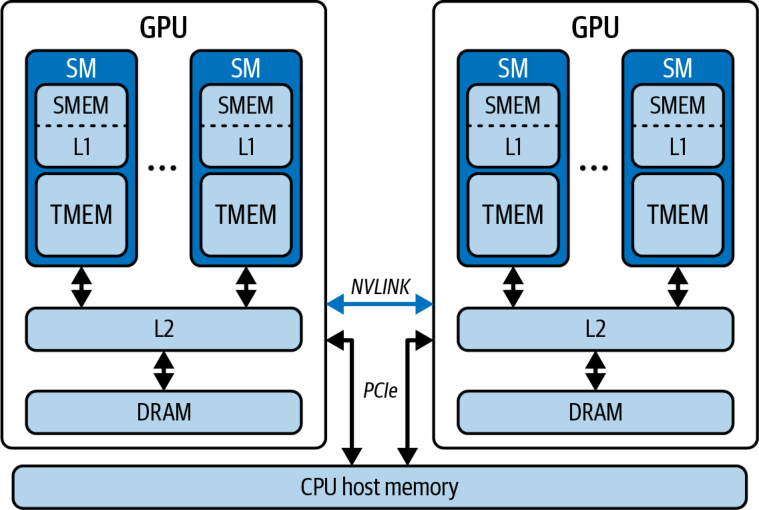
\includegraphics[width=\linewidth]{figs/fig6-10.png}\\
    {\scriptsize Figure 6-10. GPU memory hierarchy, including the CPU}
  \end{columns}
  \pe{your \kw{own toolbox} (registers) $\to$ the \kw{shared workbench} (shared) $\to$ the factory's \kw{central depot} (L2) $\to$ the \kw{distant warehouse} (HBM) --- do the work at your bench.}
\end{frame}

% ================================================================ 30
\begin{frame}{Register Pressure Can Turn Fast Storage into DRAM Access}
  \begin{columns}[c]
    \column{0.55\textwidth}
    \begin{itemize}
      \item Every thread ``begins its journey'' at the \kw{register file}: single-cycle reads/writes,
            contending with almost nothing --- \kw{tens of TB/s per SM}.
      \item Budget: 64K registers per SM, \kw{max 255 per thread}.
      \item The cliff: need more (too many locals, compiler temporaries) $\Rightarrow$
            overflow \kw{spills into local memory} --- which despite the name lives in
            \kw{off-chip DRAM}: hundreds to 1000+ cycles.
      \item Watch \kw{``Registers Per Thread''} in Nsight Compute --- spills are silent killers.
    \end{itemize}
    \column{0.42\textwidth}
    \centering
    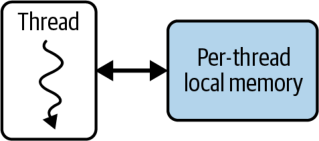
\includegraphics[width=0.6\linewidth]{figs/fig6-12.png}\\
    {\scriptsize Figure 6-12. Per-thread local memory (spill space, DRAM-backed)}
  \end{columns}
  \pe{``local memory'' is a self-storage unit across town, not your pocket.}
\end{frame}

% ================================================================ 31
\begin{frame}[fragile]{Shared Memory + L1: One SRAM, Two Jobs}
  \begin{columns}[c]
    \column{0.55\textwidth}
    \begin{itemize}
      \item One \kw{256 KB SRAM per SM}, split between user-managed \kw{shared memory}
            (up to 228 KB; 227 usable per block) and \kw{L1/data cache}.
      \item You choose the \kw{carveout}:
    \end{itemize}
\begin{lstlisting}
cudaFuncSetAttribute(myKernel,
  cudaFuncAttributePreferredSharedMemoryCarveout,
  carveoutPercent);
\end{lstlisting}
    \begin{itemize}
      \item $\sim$20--30 cycles; \kw{TB/s} if you avoid \kw{bank conflicts}
            (multiple threads hitting the same memory bank $\Rightarrow$ serialized access).
      \item This is the workbench for \kw{intrablock cooperation} --- tiles, reductions, staging.
    \end{itemize}
    \column{0.42\textwidth}
    \centering
    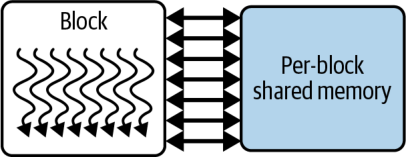
\includegraphics[width=0.75\linewidth]{figs/fig6-13.png}\\
    {\scriptsize Figure 6-13. Thread-block shared memory}
  \end{columns}
  \pe{one workbench, adjustable split: how much is your team's project table vs.\ the automatic cache shelf.}
\end{frame}

% ================================================================ 32
\begin{frame}{TMEM and TMA: Feeding the Tensor Cores}
  \begin{columns}[c]
    \column{0.55\textwidth}
    \begin{itemize}
      \item \kw{TMEM}: dedicated \kw{256 KB per-SM SRAM}, the \kw{accumulator} for 5th-gen
            Tensor Core ops (\texttt{tcgen05.*}, \kw{UMMA}); talks to Tensor Cores at tens of TB/s.
      \item \kw{Not pointer-addressable} from CUDA C++ --- data movement is orchestrated by the
            \kw{TMA} (Tensor Memory Accelerator) via \kw{descriptors}.
      \item For $C = A \times B$: operand B in SMEM, A + accumulator in TMEM; TMA moves tiles
            HBM $\to$ L2 $\to$ SMEM; SMEM $\leftrightarrow$ TMEM implicit via Tensor Core ops.
      \item Net effect: \kw{reduces Tensor Core reliance on global memory}. Details: Chapter 10.
    \end{itemize}
    \column{0.42\textwidth}
    \centering
    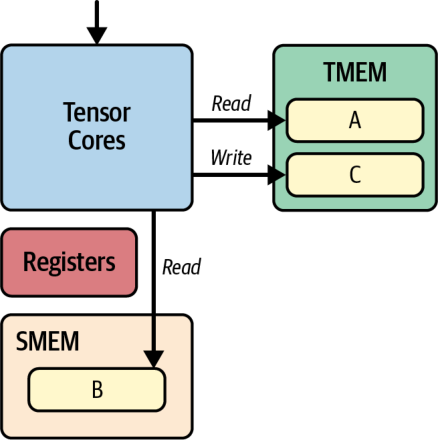
\includegraphics[width=0.72\linewidth]{figs/fig6-11.png}\\
    {\scriptsize Figure 6-11. TMEM + SMEM servicing Tensor Cores for $C = A\times B$}
  \end{columns}
  \pe{TMA is a forklift crew moving pallets in the background; the chefs never leave the kitchen.}
\end{frame}

% ================================================================ 33
\begin{frame}{Constant Cache: One-Cycle Broadcast}
  \begin{columns}[t]
    \column{0.52\textwidth}
    \begin{itemize}
      \item $\sim$\kw{8 KB cache per SM} fronting the 64 KB \kw{\texttt{\_\_constant\_\_}} space.
      \item Superpower: when all 32 threads of a warp load \kw{the same address},
            the cache \kw{broadcasts} the value in a \kw{single cycle} --- as fast as a register.
      \item Divergent reads \kw{serialize across lanes}; misses cost more --- so it's for
            \kw{small, read-only, uniformly-accessed} data.
    \end{itemize}
    \column{0.45\textwidth}
    \begin{exampleblock}{The book's LLM examples}
      \begin{itemize}\small
        \item Rotary positional encoding (RoPE) lookup tables
        \item ALiBi slopes
        \item LayerNorm $\gamma$/$\beta$ vectors
        \item Embedding quantization scales
      \end{itemize}
      \smallskip
      {\small Shared by every thread with \kw{zero global-memory traffic}.}
    \end{exampleblock}
  \end{columns}
  \pe{a megaphone, not a mailbox: one announcement reaches all 32 workers at once --- but only if they all asked the same question.}
\end{frame}

% ================================================================ 34
\begin{frame}{L2 Cache: The GPU-Wide Middleman}
  \begin{columns}[t]
    \column{0.52\textwidth}
    \begin{itemize}
      \item \kw{126 MB} shared by all SMs --- the glue between on-chip SRAM and off-chip HBM3e.
      \item $\sim$200 cycles, aggregate bandwidth in the \kw{tens of TB/s}; absorbs L1 spillover.
      \item \kw{Cross-block reuse}: data fetched by one thread block is reused by others
            \kw{without revisiting DRAM}.
    \end{itemize}
    \column{0.45\textwidth}
    \begin{block}{The coalescing rule (book tip)}
      \small Structure global loads into \kw{128-byte aligned, coalesced} segments that map
      cleanly to cache lines --- avoids split transactions, maximizes L2 \kw{and} DRAM
      bandwidth. (How-to: Chapter 7.)
    \end{block}
  \end{columns}
  \pe{L2 is the factory's \kw{central depot}: if another crew already fetched the part from the warehouse, you grab it here --- provided everyone orders \kw{whole pallets}, not single screws.}
\end{frame}

% ================================================================ 35
\begin{frame}{Global HBM3e, the Dual-Die B200, and Coherency}
  \begin{columns}[c]
    \column{0.55\textwidth}
    \begin{itemize}
      \item \kw{180 GB} on B200 ($\sim$288 GB on B300) at \kw{$\sim$8 TB/s} --- but
            \kw{hundreds to 1000+ cycles}: the slowest link in the chain.
      \item Register spills and oversized automatic arrays (local memory) also pay this price.
      \item \kw{Fun fact (book note)}: B200 = \kw{two reticle-limited dies} joined by a
            \kw{10 TB/s} chip-to-chip interconnect, 4 HBM3e stacks each ---
            presented to you as \kw{one GPU, one address space}.
      \item \kw{Point of coherency} (Figure 6-15): memory consistency is established at
            thread $\to$ block $\to$ cluster $\to$ device $\to$ system scope ---
            the wider the communication, the higher the cost.
    \end{itemize}
    \column{0.42\textwidth}
    \centering
    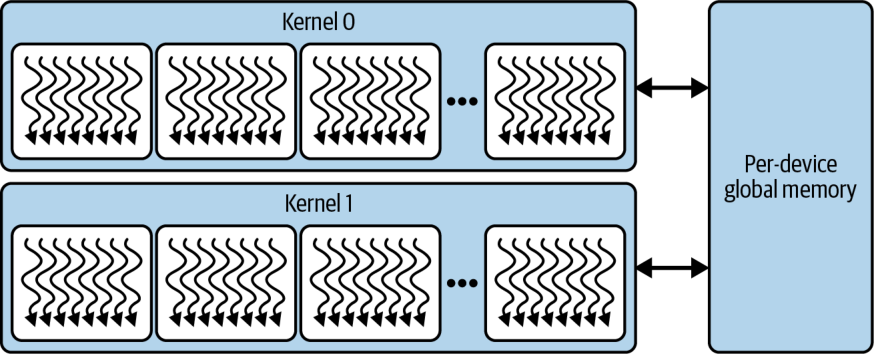
\includegraphics[width=\linewidth]{figs/fig6-14.png}\\[2pt]
    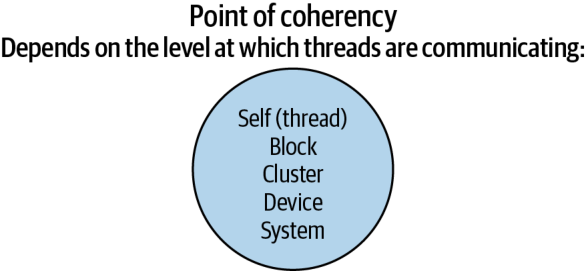
\includegraphics[width=0.9\linewidth]{figs/fig6-15.png}\\
    {\scriptsize Figures 6-14 / 6-15. Global memory; points of coherency}
  \end{columns}
\end{frame}

% ================================================================ 36
\begin{frame}{Unified Memory Hides Copies, Not Their Cost}
  \begin{columns}[c]
    \column{0.55\textwidth}
    \begin{itemize}
      \item \kw{\texttt{cudaMallocManaged()}}: one coherent CPU+GPU address space ---
            no separate buffers, no manual \texttt{cudaMemcpy}.
      \item Under the hood: pages \kw{migrate on demand} over whatever link connects CPU and GPU.
      \item The catch: a GPU touch of a CPU-resident page \kw{page-faults and stalls the kernel}.
      \item On PCIe: on-fault transfers can be \kw{slower than manual memcpy}.
            On Grace superchips, \kw{NVLink-C2C} ($\sim$900 GB/s) makes migrations near
            device-native --- \kw{but latency is never zero}.
    \end{itemize}
    \column{0.42\textwidth}
    \centering
    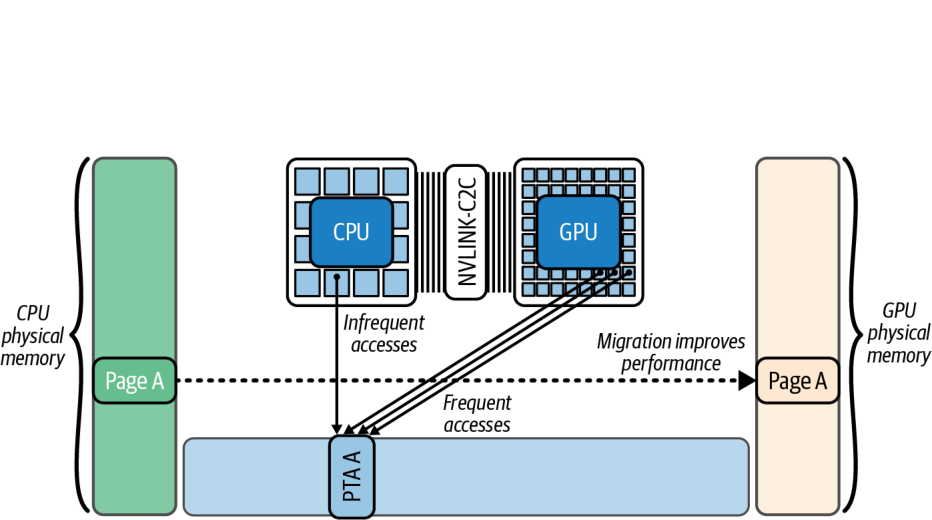
\includegraphics[width=\linewidth]{figs/fig6-16.png}\\
    {\scriptsize Figure 6-16. Automatic page migration with Unified Memory}
  \end{columns}
  \pe{Unified Memory is \kw{automatic parts delivery}: convenient --- but if the part isn't in the workshop when the crew needs it, \kw{the crew stands and waits}.}
\end{frame}

% ================================================================ 37
\begin{frame}[fragile]{Taming Unified Memory: Prefetch, Advise, Attach}
  \begin{columns}[t]
    \column{0.55\textwidth}
\begin{lstlisting}
// 1) move data BEFORE the kernel needs it:
cudaMemPrefetchAsync(ptr, size, gpuId, s);
// 2) tell the driver how you'll use it:
cudaMemAdvise(ptr, size,
    cudaMemAdviseSetPreferredLocation, gpuId);
cudaMemAdvise(ptr, size,
    cudaMemAdviseSetReadMostly, gpuId);
cudaMemAdvise(ptr, size,
    cudaMemAdviseSetAccessedBy, otherGpuId);
// 3) confine faults/migrations to one stream:
cudaStreamAttachMemAsync(stream, ptr, 0,
    cudaMemAttachSingle);
\end{lstlisting}
    \column{0.42\textwidth}
    \begin{itemize}\small
      \item \kw{Prefetch} turns first-touch migrations into \kw{overlappable async transfers}
            (Figure 6-17).
      \item \kw{ReadMostly} allows replicated read-only copies; \kw{AccessedBy} lets a second GPU
            map pages \kw{without} migration (Figure 6-18).
      \item \kw{Attach} stops \emph{other} streams from stalling on this range.
      \item No NVLink-C2C? Pin data \kw{NUMA-local} (peer copy / prefetch).
      \item Result: performance \kw{close to manual \texttt{cudaMemcpy}}, simplicity retained.
    \end{itemize}
  \end{columns}
\end{frame}

% ================================================================ 38
\begin{frame}{Part IV --- Occupancy Ground Rules}
  \bridge{The memory ladder explains \emph{why} warps stall. Occupancy asks: how many \emph{other} warps do we need to fill those gaps?}
  \begin{block}{The most fundamental rule of CUDA performance (book)}
    \centering \kw{``Launch enough parallel work to fully occupy the GPU.''}
  \end{block}
  \begin{columns}[t]
    \column{0.48\textwidth}
    \begin{block}{Rule 1 --- low occupancy, poor perf}
      \small First remedy: \kw{increase parallelism} (more blocks/threads) until there are
      \kw{enough ready warps to hide latency} --- stop when performance \kw{plateaus}.
    \end{block}
    \column{0.48\textwidth}
    \begin{block}{Rule 2 --- occupancy already high}
      \small If the kernel is \kw{memory-bound}, pushing to 100\% won't help: you need
      \kw{just enough warps to hide latency} --- beyond that, the bottleneck is bandwidth.
    \end{block}
  \end{columns}
  \medskip
  \begin{itemize}\small
    \item Up next: one operation ($C = A + B$, $N = 10^6$), two implementations,
          and what the profilers say about them.
  \end{itemize}
  \pe{rule 1 \kw{fills the workshop with crews}; rule 2: a full workshop \kw{still stalls} if the warehouse truck is the bottleneck.}
\end{frame}

% ================================================================ 39
\begin{frame}[fragile]{Case Study, Take 1: addSequential}
  \begin{columns}[t]
    \column{0.52\textwidth}
\begin{lstlisting}
// Single thread does ALL N additions
__global__ void addSequential(const float* A,
    const float* B, float* C, int N) {
  if (blockIdx.x == 0 && threadIdx.x == 0) {
    for (int i = 0; i < N; ++i) {
      C[i] = A[i] + B[i];
    }
  }
}
// Note: this kernel assumes <<<1,1>>>.
addSequential<<<1,1>>>(d_A, d_B, d_C, N);
cudaDeviceSynchronize();
\end{lstlisting}
    \column{0.44\textwidth}
    \begin{itemize}
      \item One thread, one warp, one SM --- \kw{everything else watches}.
      \item Book: ``the GPU's vast resources are mostly idle... very poor occupancy and,
            ultimately, low performance.''
      \item No other warps to switch to $\Rightarrow$ memory waits become
            \kw{pure idle time} --- zero latency hiding.
    \end{itemize}
  \end{columns}
  \pe{you rented the whole factory and hired one worker.}
\end{frame}

% ================================================================ 40
\begin{frame}[fragile]{The Same Trap in PyTorch}
  \begin{columns}[t]
    \column{0.52\textwidth}
\begin{lstlisting}[language=Python]
import torch
N = 1_000_000
A = torch.arange(N, dtype=torch.float32,
                 device='cuda')
B = 2 * A
C = torch.empty_like(A)
torch.cuda.synchronize()
# Naive, sequential GPU ops - DO NOT DO THIS
with torch.inference_mode():
    for i in range(N):     # N tiny serial kernels!
        C[i] = A[i] + B[i]
torch.cuda.synchronize()
\end{lstlisting}
    \column{0.44\textwidth}
    \begin{itemize}
      \item A Python loop around GPU ops \kw{serializes N tiny kernel launches} ---
            the GPU becomes ``a scalar, nonparallel processor.''
      \item Same terrible occupancy, plus \kw{per-launch CPU overhead} $\times$ 1{,}000{,}000.
      \item Book advice: there is \kw{almost always an optimized PyTorch-native
            (vectorized) implementation} --- including compiler-emitted code.
    \end{itemize}
  \end{columns}
  \pe{the most common GPU bug: accidentally using the GPU as a very expensive single-core CPU.}
\end{frame}

% ================================================================ 41
\begin{frame}[fragile]{Case Study, Take 2: addParallel --- and \texttt{C = A + B}}
  \begin{columns}[t]
    \column{0.52\textwidth}
\begin{lstlisting}
// One thread per element
__global__ void addParallel(
    const float* __restrict__ A,
    const float* __restrict__ B,
    float* __restrict__ C, int N) {
  int idx = blockIdx.x*blockDim.x + threadIdx.x;
  if (idx < N) C[idx] = A[idx] + B[idx];
}
addParallel<<<(N+255)/256, 256>>>(dA, dB, dC, N);
\end{lstlisting}
    {\small The book's full version also uses pinned host memory, a non-blocking stream, and
    \texttt{cudaMallocAsync}/\texttt{cudaMemcpyAsync} --- the habits from Part II.}
    \column{0.44\textwidth}
    \begin{itemize}
      \item $\sim$3{,}907 blocks $\times$ 256 threads --- \kw{a million threads} cover the array
            (Figure 6-19).
      \item \kw{\texttt{\_\_restrict\_\_}}: promises no pointer aliasing --- frees the compiler
            to optimize.
      \item PyTorch equivalent is one line: \kw{\texttt{C = A + B}} ---
            a single vectorized kernel engaging many threads concurrently.
    \end{itemize}
  \end{columns}
  \pe{same factory, now every workstation is staffed --- and the PyTorch version is just ``hire the staffing agency.''}
\end{frame}

% ================================================================ 42
\begin{frame}[fragile]{Measuring It: nsys and ncu}
  \begin{columns}[t]
    \column{0.55\textwidth}
\begin{lstlisting}[language=bash]
# Nsight Systems: whole-app timeline
nsys profile --stats=true -t cuda,nvtx \
     -o report ./add_parallel.py

# Nsight Compute: per-kernel counters
ncu --section SpeedOfLight \
    --metrics sm__warps_active.avg.\
pct_of_peak_sustained_active,gpu__time_duration.avg \
    --target-processes all \
    --print-summary per-gpu -o report ./add_parallel.py
\end{lstlisting}
    \column{0.42\textwidth}
    \begin{itemize}
      \item \kw{nsys} answers ``\kw{where does time go} --- is the GPU starved or blocked?''
      \item \kw{ncu} answers ``\kw{why is this kernel slow} --- occupancy? stalls? cache misses?''
      \item Run \kw{both}: nsys alone misses in-kernel inefficiency; ncu alone can't see
            whether kernels are \kw{fed data fast enough}.
      \item That long \texttt{sm\_\_warps\_active...} metric \kw{is} achieved occupancy.
    \end{itemize}
  \end{columns}
  \pe{nsys is the stopwatch for the whole machine; ncu is the microscope on one kernel.}
\end{frame}

% ================================================================ 43
\begin{frame}{Parallelism Cuts Runtime 22$\times$ at Only 38.7\% Occupancy}
  \begin{columns}[c]
    \column{0.52\textwidth}
    {\small
    \begin{tabular}{@{}lrr@{}}
      \toprule
      \textbf{Metric} & \textbf{Sequential} & \textbf{Parallel} \\
      \midrule
      Kernel time (ms) & 48.21 & \kw{2.17} \\
      GPU utilization & 1.5\% & \kw{95\%} \\
      Achieved occupancy & 1.3\% & \kw{38.7\%} \\
      Warp exec.\ efficiency & 3.1\% & \kw{100\%} \\
      \bottomrule
    \end{tabular}}\\[4pt]
    {\scriptsize Table 6-6 (illustrative --- real benchmarks in the book's repo\refmark{7}).
    Warp efficiency 3.1\% $\approx$ 1/32: one active lane per warp.}
    \column{0.45\textwidth}
    \centering
    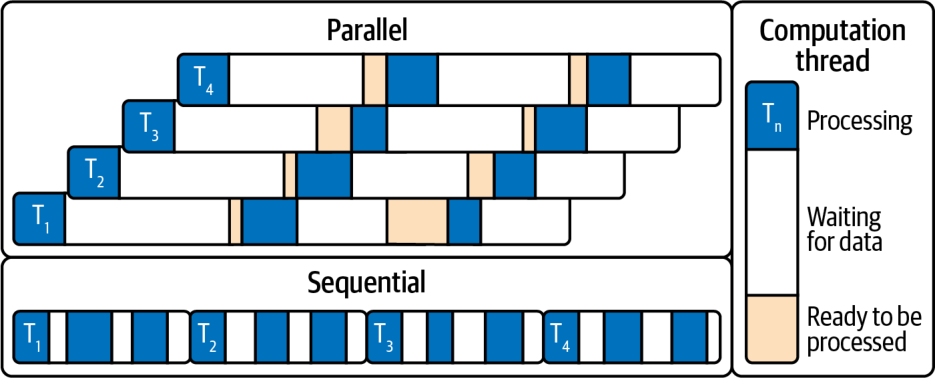
\includegraphics[width=\linewidth]{figs/fig6-20.png}\\
    {\scriptsize Figure 6-20. Sequential timeline has idle gaps; in the parallel version other
    warps' work fills them}
  \end{columns}
  \medskip
  \begin{itemize}\small
    \item Note: 38.7\% occupancy already bought 22$\times$ --- you don't need 100\%.
    \item GPU utilization, SM active \%, achieved occupancy, and warp efficiency are
          \kw{related but different metrics} --- which is exactly how
          \kw{95\%}, \kw{38.7\%}, and \kw{100\%} coexist on one kernel.
  \end{itemize}
\end{frame}

% ================================================================ 44
\begin{frame}{A Busy GPU Can Still Be Waiting on Memory (LLM Decode)}
  \bridge{95\% utilization at only 38.7\% occupancy, already 22$\times$ faster --- so we don't need 100\%. But are we at peak FLOPS? No: vector add mostly \emph{moves data}.}
  \vspace{-4pt}
  \begin{itemize}\small
    \item After parallelism, the next lever is per-warp efficiency (ILP etc., Chapter 8). But:
          \kw{even at 100\% occupancy}, performance suffers if the kernel is
          \kw{memory bound} --- limited by data movement, not compute.
    \item The book's canonical example: the \kw{decode phase of an LLM} ---
          every generated token streams \kw{model weights} from HBM into registers/shared memory.
    \item Hundreds of billions of parameters $\times$ $\sim$1 byte $\approx$
          \kw{hundreds of GB} per pass --- this \kw{saturates memory bandwidth} regardless
          of thread count.
  \end{itemize}
  \begin{block}{The trend that makes this worse (book note)}
    \kw{GPU FLOPS are outpacing memory bandwidth.} Blackwell HBM3e delivers $\sim$8 TB/s,
    but compute and model sizes grow faster --- \kw{optimizing memory movement is absolutely
    critical} in modern AI workloads.
  \end{block}
  \pe{when the whole job is ``carry boxes from the warehouse,'' hiring more clerks at the desk doesn't help --- that's what the roofline model (Part V) formalizes.}
\end{frame}

% ================================================================ 45
\begin{frame}[fragile]{\texttt{\_\_launch\_bounds\_\_}: Compile-Time Occupancy Control}
  \begin{columns}[t]
    \column{0.5\textwidth}
\begin{lstlisting}
// promise: never launched with > 256 thr/block
// request: keep >= 16 blocks resident per SM
__global__ __launch_bounds__(256, 16)
void myKernel(...) { /* ... */ }
\end{lstlisting}
    \begin{itemize}\small
      \item 16 $\times$ 256 = 4{,}096 $>$ 2{,}048 limit $\Rightarrow$ compiler \kw{clamps} to
            8 blocks and warns:\\
            {\scriptsize\texttt{ptxas warning: ... .minnctapersm will be ignored}}
    \end{itemize}
    \column{0.47\textwidth}
    \begin{itemize}
      \item Effect: compiler \kw{caps per-thread registers} (and may restrict unrolling/inlining)
            to avoid spills and fit \kw{more warps per SM}.
      \item The deal: trade a bit of \kw{per-thread performance} for
            \kw{more consistent warp throughput} (more warps in flight).
      \item Danger zone: forcing too many threads $\Rightarrow$ registers run out $\Rightarrow$
            \kw{spilling to local memory} --- slower than what you started with.
    \end{itemize}
  \end{columns}
  \pe{you're trading each worker's toolbox size for the number of workers on the floor --- the sweet spot is empirical.}
\end{frame}

% ================================================================ 46
\begin{frame}[fragile]{The Occupancy API: Runtime Autotuning}
  \begin{columns}[t]
    \column{0.55\textwidth}
\begin{lstlisting}
int minGridSize = 0, bestBlockSize = 0;
// if kernel uses extern __shared__, set truthfully:
size_t dynSmemBytes = 0;
cudaOccupancyMaxPotentialBlockSize(
    &minGridSize, &bestBlockSize, myKernel,
    dynSmemBytes, /*blockSizeLimit=*/0);
// cover N, but don't go below the min grid
// that saturates occupancy:
int gridSize = std::max(minGridSize,
    (N + bestBlockSize - 1) / bestBlockSize);
myKernel<<<gridSize, bestBlockSize,
           dynSmemBytes>>>(...);
\end{lstlisting}
    \column{0.42\textwidth}
    \begin{itemize}
      \item Computes the block size that \kw{maximizes occupancy} given the kernel's actual
            register/shared-memory usage.
      \item Two gotchas (book): \kw{\texttt{minGridSize}} saturates occupancy ---
            it is \kw{not} the grid that covers N (take the \texttt{max}); and
            \kw{pass real dynamic shared-memory bytes}.
      \item Book tip: \kw{validate with $\pm$1--2 candidate block sizes} --- register pressure and
            L2 behavior can make slightly \kw{sub-maximal occupancy faster}.
    \end{itemize}
  \end{columns}
\end{frame}

% ================================================================ 47
\begin{frame}{Part V --- Debugging Correctness: NVIDIA Compute Sanitizer}
  \bridge{No more blind-tuning block sizes --- next: compute ceiling or memory ceiling? (roofline, after a correctness detour)}
  \vspace{-4pt}
  \begin{columns}[t]
    \column{0.48\textwidth}
    \begin{block}{Memory}
      \begin{itemize}\small
        \item \kw{memcheck} --- out-of-bounds / misaligned accesses (global, local, shared),
              HW exceptions, device leaks; \texttt{--check-device-heap}.
        \item \kw{initcheck} --- reads of uninitialized global memory
              (classic cause: a \kw{missing H2D copy}).
      \end{itemize}
    \end{block}
    \column{0.48\textwidth}
    \begin{exampleblock}{Concurrency}
      \begin{itemize}\small
        \item \kw{racecheck} --- shared-memory hazards: \kw{WAW / WAR / RAW}
              $\Rightarrow$ nondeterministic behavior.
        \item \kw{synccheck} --- invalid sync primitives, mismatched barriers
              $\Rightarrow$ deadlocks, inconsistent state.
      \end{itemize}
    \end{exampleblock}
  \end{columns}
  \begin{itemize}\small
    \item CLI: \texttt{compute-sanitizer [--tool <name>] <app>}; filter with
          \texttt{--kernel-name}, annotate with \kw{NVTX} (\texttt{--nvtx yes}).
    \item Book tip: run it in \kw{CI} with \kw{\texttt{--error-exitcode}}.\refmark{5}
  \end{itemize}
  \pe{``it works on my run'' means nothing at 100{,}000 threads --- the sanitizer is your seatbelt.}
\end{frame}

% ================================================================ 48
\begin{frame}{Roofline Tells Us Which Resource Is the Limit}
  \begin{columns}[c]
    \column{0.5\textwidth}
    \begin{itemize}
      \item \kw{Arithmetic intensity} = FLOPs per byte moved to/from HBM.
      \item Two ceilings: \kw{flat} compute roof ($\sim$80 TFLOP/s FP32) and \kw{sloped}
            memory roof ($\sim$8 TB/s), crossing at the \kw{ridge point} $\approx$
            \kw{10 FLOPs/byte} (80T $\div$ 8T).
      \item Worked example: $C = A + B$ loads 8 B, adds once, stores 4 B $\Rightarrow$
            1 FLOP / 12 B $=$ \kw{0.083 FLOPs/byte} --- $>$100$\times$ left of the ridge:
            hopelessly \kw{memory-bound}.
      \item Book note: LLMs are \kw{both} --- \kw{prefill} tends compute-bound,
            \kw{decode} tends memory-bound (Ch.\ 15--18).
    \end{itemize}
    \column{0.47\textwidth}
    \centering
    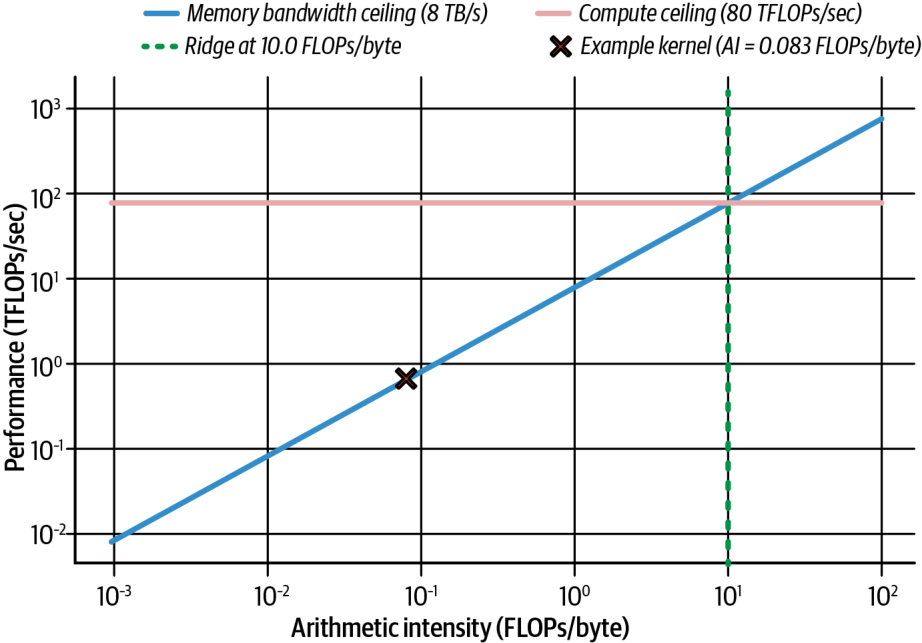
\includegraphics[width=\linewidth]{figs/fig6-21.png}\\
    {\scriptsize Figure 6-21. Roofline for a Blackwell-class GPU; our kernel sits at 0.083 FLOPs/byte}
  \end{columns}
  \pe{the roofline asks first: is this kernel \kw{starving for math, or for data}?\refmark{4}}
\end{frame}

% ================================================================ 49
\begin{frame}{Moving Right on the Roofline: Lower Precision Pays Twice}
  \begin{itemize}
    \item To escape the memory-bound region, \kw{do more work per byte}: reuse data on-chip,
          fuse ops --- or simply \kw{shrink the bytes}.
    \item One 128-byte transaction carries \kw{32 FP32 = 64 FP16 = 128 FP8 = 256 FP4} values.
          FP32 $\to$ FP16 instantly \kw{doubles} FLOPs/byte; FP8 doubles throughput and halves
          memory again vs.\ FP16.
    \item Blackwell adds native \kw{FP8 and FP4 Tensor Cores}, plus \kw{hardware decompression}:
          weights stored compressed in HBM (even beyond FP4 --- 4-bit/2-bit schemes) are expanded
          on the fly and cast to FP16/FP32 for accurate accumulation.
    \item Net: \kw{effectively more memory bandwidth} --- an architectural edge for
          memory-bound \kw{token generation}.
  \end{itemize}
  \medskip
  \begin{block}{The takeaway}
    Precision is a \kw{bandwidth} optimization as much as a compute one:
    halve the bytes $\Rightarrow$ double the arithmetic intensity $\Rightarrow$ move toward the compute roof.
  \end{block}
\end{frame}

% ================================================================ 50
\begin{frame}{Profiling Workflow: Diagnose, Fix, Re-measure}
  \begin{columns}[c]
    \column{0.52\textwidth}
    \begin{itemize}\small
      \item Memory-bound signature in \kw{ncu}: \kw{high DRAM utilization + low ALU utilization}
            --- warps stalled on memory. Also watch \kw{global load efficiency} dropping.
      \item \kw{nsys} timeline shows idle stretches between kernels = GPU waiting on transfers.
      \item Expected overlap but see sequential copy-then-kernel? Two usual suspects:
            an unwanted \kw{default-stream sync}, or a \kw{missing pinned-memory buffer} ---
            without pinned memory, \texttt{cudaMemcpyAsync} \kw{cannot overlap} with kernels.
      \item Newer ncu niceties: \kw{range replay}, source correlation, launch-stack size metric.
      \item After fixes: idle gaps vanish, \kw{memory pipe utilization} climbs toward peak.
    \end{itemize}
    \column{0.45\textwidth}
    \centering
    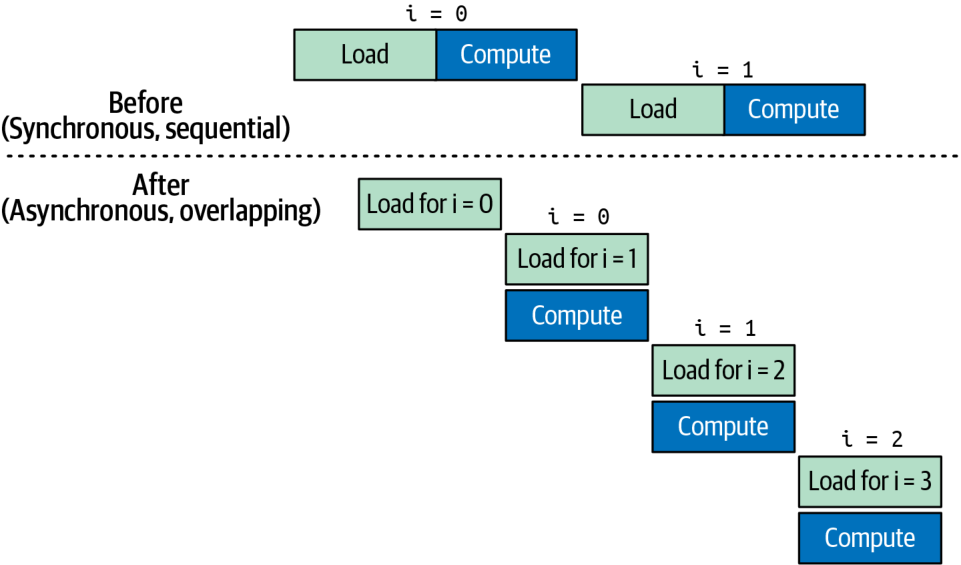
\includegraphics[width=\linewidth]{figs/fig6-22.png}\\
    {\scriptsize Figure 6-22. Sync (sequential) vs.\ async (overlapped) transfers + compute}
    \smallskip
    {\footnotesize\itshape Always measure after each change --- profilers confirm whether stalls actually dropped.}
  \end{columns}
\end{frame}

% ================================================================ 51
\begin{frame}{Key Takeaways (the Book's Eight)}
  \begin{columns}[t]
    \column{0.48\textwidth}
    \begin{itemize}\small
      \item \kw{SIMT}: 32-thread warps in lockstep; many warps in flight = latency hidden.
      \item \kw{Hierarchy}: threads $\to$ blocks ($\leq$1{,}024) $\to$ grids; minimize
            \texttt{\_\_syncthreads()} barriers.
      \item \kw{Occupancy vs.\ limits}: multiples of 32; per-SM: 64 warps, 32 blocks,
            228 KB shared, 255 regs/thread.
      \item \kw{Launch params}: 256 threads/block to start; grid = ceil(N/256);
            tune via profiling.
    \end{itemize}
    \column{0.48\textwidth}
    \begin{itemize}\small
      \item \kw{Async memory}: \texttt{cudaMallocAsync} + streams + pools;
            PyTorch's caching allocator ditto.
      \item \kw{Memory ladder}: reuse in registers/shared/L1; coalesce into L2/HBM.
      \item \kw{Unified Memory}: prefetch + advise to kill surprise stalls.
      \item \kw{Roofline}: FLOPs/byte picks your battle; FP16/FP8/FP4 + hardware decompression
            move you right; \kw{TMEM + UMMA} can shift kernels memory- $\to$ compute-bound.
    \end{itemize}
  \end{columns}
\end{frame}

% ================================================================ 52
\begin{frame}{Conclusion and What's Next}
  \begin{block}{This chapter in one sentence}
    Make the GPU \kw{busy} (occupancy), make data \kw{close} (memory hierarchy),
    and let the \kw{roofline} tell you which battle to fight next.
  \end{block}
  \begin{itemize}
    \item The book's closing caveat: \kw{max occupancy is not always optimal} ---
          with enough \kw{ILP} per thread, moderate/low occupancy can win; sometimes
          \kw{fewer threads with more registers each} is faster. \kw{Always benchmark.}
    \item Coming next in the book: warp divergence \& memory-access tuning (Ch.\ 7--8),
          arithmetic intensity (Ch.\ 9), TMA \& warp specialization (Ch.\ 10).
    \item My second talk --- \kw{Chapter 12} --- builds on this: once single kernels are fast,
          how do we \kw{orchestrate} them so the GPU never waits for the CPU?
  \end{itemize}
  \medskip
  \centering\itshape Questions?
\end{frame}

% ================================================================ 53
\begin{frame}{References \& Further Reading}
  \begingroup\footnotesize
  \begin{enumerate}
    \item C.\ Fregly. \emph{AI Systems Performance Engineering} (O'Reilly, 2026), Chapter 6.
    \item NVIDIA. \emph{Blackwell Tuning Guide} and \emph{Blackwell Architecture Whitepaper} ---
          SM limits, dual-issue schedulers, TMEM/tcgen05.
    \item NVIDIA. \emph{CUDA C++ Programming Guide} --- thread hierarchy, Unified Memory,
          occupancy API, \texttt{\_\_launch\_bounds\_\_}, stream-ordered allocation, PTX/fatbin.
    \item S.\ Williams, A.\ Waterman, D.\ Patterson. \emph{Roofline: An Insightful Visual Performance
          Model for Multicore Architectures}. CACM 52(4), 2009.
    \item NVIDIA. \emph{Compute Sanitizer User Guide} --- memcheck, racecheck, initcheck, synccheck.
    \item NVIDIA. \emph{Nsight Systems} and \emph{Nsight Compute} documentation ---
          \texttt{nsys profile}, \texttt{ncu --section SpeedOfLight}, NVTX.
    \item Book code and benchmarks: the book's GitHub repository (per-architecture results for the
          illustrative tables in this deck).
  \end{enumerate}\endgroup
\end{frame}

\end{document}
